\documentclass[a4paper]{article}

\pdfmajorversion=1
\pdfminorversion=7
\pdfcompresslevel=9
\pdfobjcompresslevel=2

\usepackage[hidelinks]{hyperref}
\usepackage[margin=60pt]{geometry}
\usepackage[utf8]{inputenc}
\usepackage[english]{babel}
\usepackage{colortbl}
\usepackage{graphicx}
\usepackage{subcaption}
\usepackage{tabularx}
\usepackage{xcolor}

\setlength{\parindent}{0pt}

\hypersetup{
    pdftitle={Formal Digital Twin of a LEGO® MINDSTROMS™ Production Plant},
    pdfauthor={Andrea Infantino, Riccardo Motta, Matteo Negro}
}

\captionsetup[figure]{labelfont=bf}

\newcommand{\figureref}[1]{Figure \ref{#1}}
\newcommand{\reference}[1]{\ref{#1}: \nameref{#1} (page \pageref{#1})}
\newcommand{\nbvspace}[1][3]{\vspace*{\stretch{#1}}}

\renewcommand\tabularxcolumn[1]{m{#1}}

\arrayrulecolor{lightgray}

\begin{document}

    \begin{titlepage}

        \begin{center}

            \nbvspace[1]

            
\includegraphics[width=0.3\columnwidth]{./images/polimi}

            \nbvspace[2]

            {\huge \textbf{\textsc{Formal Digital Twin of a \\ LEGO\textsuperscript{\textregistered} MINDSTROMS\texttrademark \\\medskip Production Plant}}} \\
            [3em]
            {\Large Formal Methods for Concurrent and Real-Time Systems} \\
            [1.5em]
            {\Large A.Y. 2022-2023}

            \nbvspace[8]

            \begin{tabular}{lrp{0.04\columnwidth}lrp{0.04\columnwidth}lr}
                \multicolumn{2}{c}{\large \textbf{Andrea Infantino}} & & \multicolumn{2}{c}{\large \textbf{Riccardo Motta}} & & \multicolumn{2}{c}{\large \textbf{Matteo Negro}} \\
                Person ID & 10671720 & & Person ID & 10658639 & & Person ID & 10642961 \\
                Student ID & 225757 & & Student ID & 218685 & & Student ID & 222025
            \end{tabular}

            \nbvspace[1]

        \end{center}

    \end{titlepage}

    \tableofcontents{}

    \pagebreak

    \section{Model Description}

    This section provides a description of the production plant with some implementation details, together with all the components that make it up. The motivations behind these modelling choices can be found in Section \reference{section:design_decisions}.

    \subsection{The Production Plant}

    \begin{figure}[h!]
        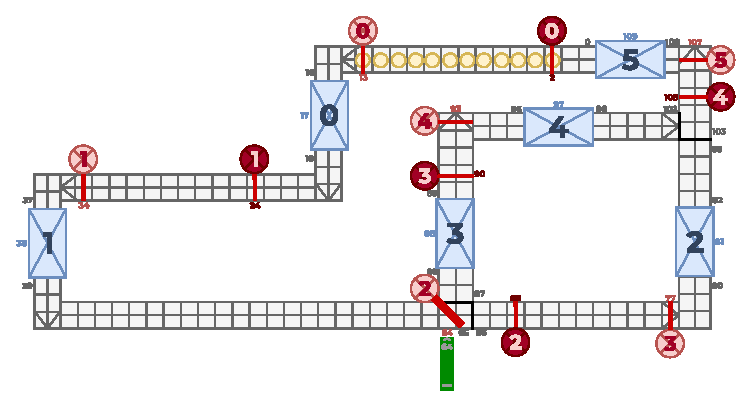
\includegraphics[width=\columnwidth]{./images/plant}
        \caption{the production plant we modelled.}
        \label{figure:scheme}
    \end{figure}

    This is the plant we modelled in our project. The yellow circles are the workpieces, the blue rectangles are the processing stations, the light and dark red circles are the sensors and the green bar is the flow controller.

    \paragraph{Notes on the scheme} We enhanced the original scheme with the number the various stations and laser sensors have inside our project and with the numbers of the positions of the conveyor belt, in order to respect what we have done inside the project.

    \subsection{General Overview}

    The model of our system is made of 6 different components which interact between them in order to coordinate the entire production plant. Some of them are also instantiated many times in order to have a simpler modelling of the entire system.

    \paragraph{Initializer} It's a fictitious component which represents the entry point of the whole system. It allows us to instantiate all the workpieces in the correct positions of the conveyor belt (positions which start from position 13 and ends in position 2 in our model) and works as the general clock of the system.

    \paragraph{Motor} This is the real motor of the system. According to the speed at which the conveyor belt should be moving, uses the clock to make all the workpieces move and synchronizes the whole system.

    \paragraph{Conveyor belt} It's the set of all the various conveyor belts of the plant. It's the one in charge of moving around all the workpieces. In our model it's also the one in charge of blocking workpieces and stations from proceeding according to the pieces of information gathered by the laser sensors and the stations and also manages the positions where the two branches of the plant start and merge.

    \paragraph{Processing stations} They are the ones in charge of processing the various workpieces one they get into them. We have a single template for them which is instantiated as many times as needed in order to recreate the plant. They have all a position on the conveyor belt which is managed in a special way.

    \paragraph{Laser sensors} We have modelled them in two different ways according to their functionalities. The ones guarding the entrance of a station are called \texttt{InSensor}, while the ones guarding the queue and preventing the station right before it to release a workpiece are called \texttt{OutSensor}. Like the stations, they are represented as a single template (one for each type) instantiated multiple times.

    \paragraph{Flow controller} This is the green piece of \figureref{figure:scheme}. It is pre-configured with a specific policy (which is customizable) and decides whether to send the workpieces once they get at position 65 of the conveyor belt. The available policies are the following ones:
    \begin{enumerate}
        \item[0.] Sends the workpieces on the alternative branch until its queue is full, otherwise lets the workpieces proceed on the main branch;
        \item[1.] Lets all the workpieces to flow on the main branch;
        \item[2.] Sends all the workpieces on the alternative branch;
        \item[3.] Every time a workpiece is in front of him sends it on a different path with respect to the one taken by the previous workpiece.
    \end{enumerate}

    \subsection{Initializer (\texttt{Initializer})}

    \begin{figure}[h!]
        \centering
        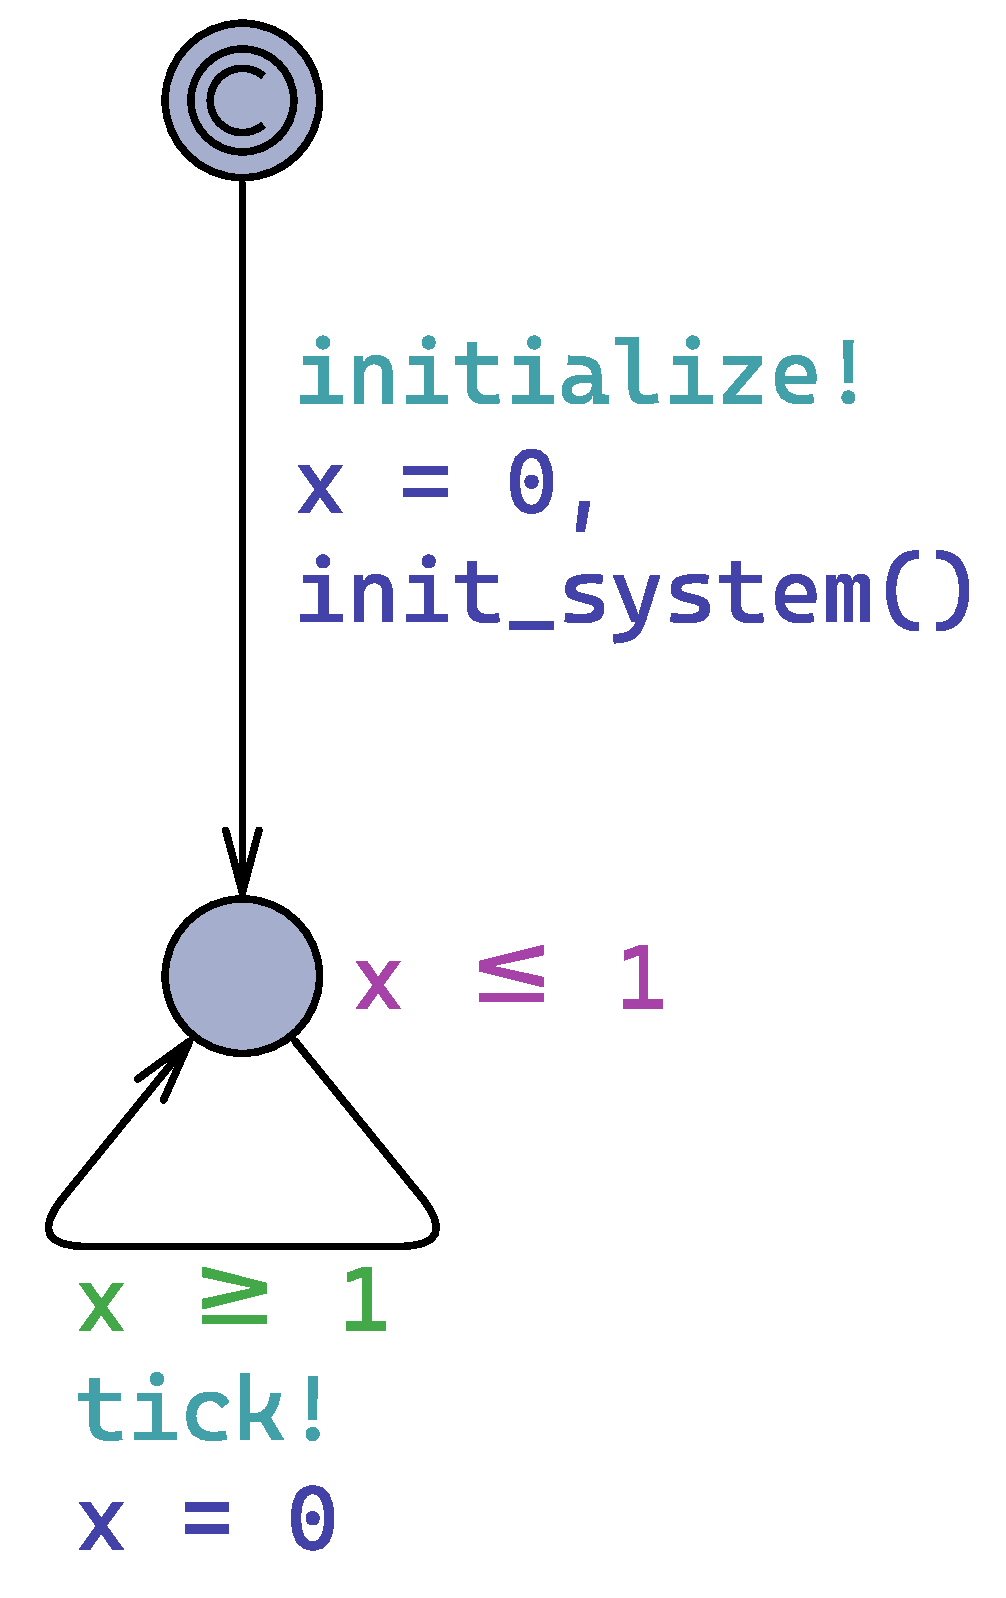
\includegraphics[width=0.12\columnwidth]{./images/automata/initializer}
        \caption{the Timed Automata of the initializer.}
    \end{figure}

    The initializer is a meta component that performs two different actions on the system and is the fundamental entry point of our whole modelling.

    \paragraph{Initialization} Initializes the system by placing the workpieces starting from the in sensor of the first station (index 0) backward with an upper limit of 12 workpieces.

    \paragraph{Global synchronization} In order to have a simpler model to verify, we decided to have a unique clock for the whole system. This TA performs as the general clock and all the components of our plant directly or indirectly synchronizes with it (usually by means of the signals generated by the motor).

    \subsection{Motor (\texttt{Motor})}

    \begin{figure}[h!]
        \centering
        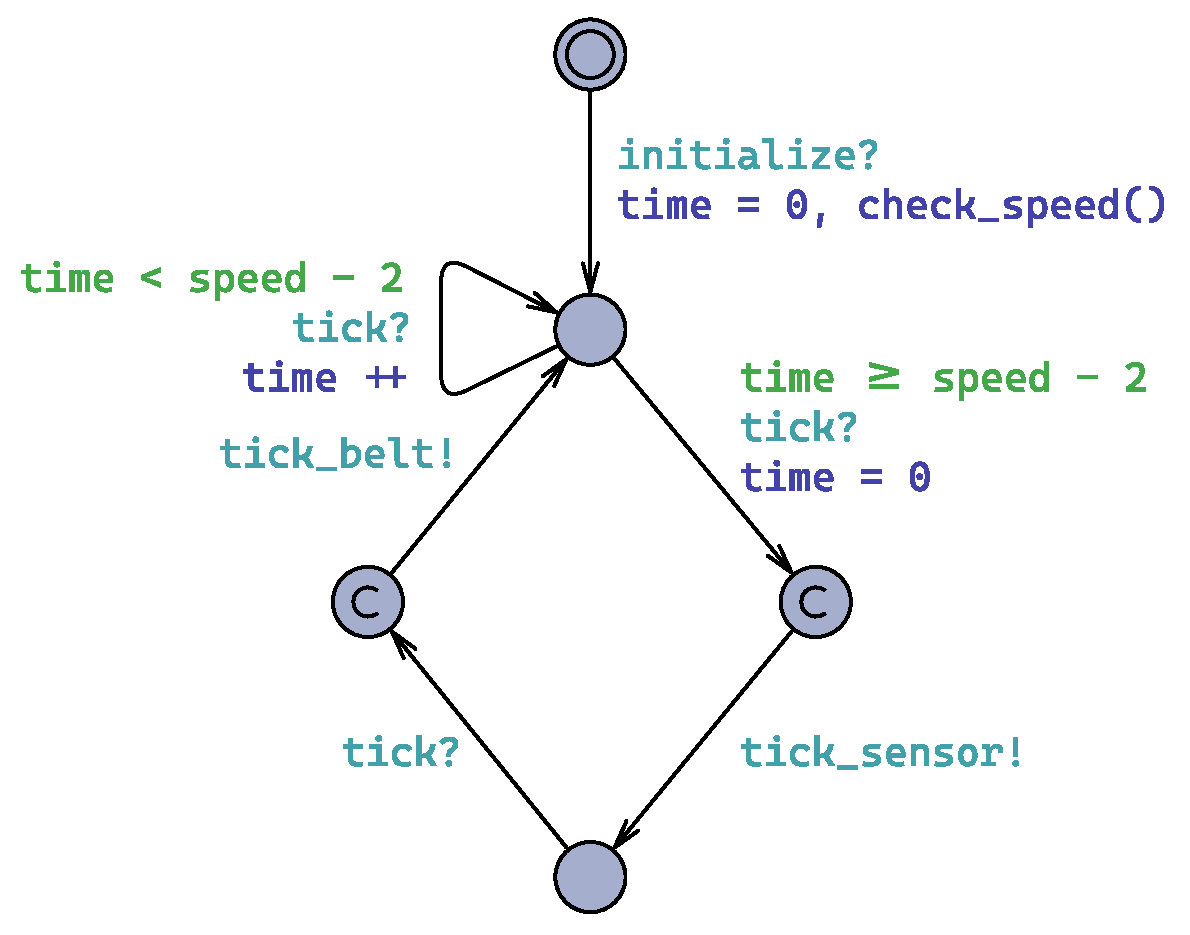
\includegraphics[width=0.3\columnwidth]{./images/automata/motor}
        \caption{the Timed Automata of the motor.}
    \end{figure}

    As the name says, this is the meta component that manages all the signals used by the sensors and, especially, the conveyor belt and the stations in order to synchronize the movement of the workpieces. The two signals which it generates are presented here.

    \paragraph{Conveyor belt's tick (\texttt{tick\_belt}, also used by the stations)} It's the signal which makes the conveyor belt move all the workpieces it can one step forward (taking into account also the branch in the conveyor belt).

    \paragraph{Laser sensors and stations' tick (\texttt{tick\_sensor})} In order to avoid any potential race condition, we decided to send a signal right before \texttt{tick\_belt}. This allows us to update the state of the laser sensors (i.e., they can check if there is a workpiece right below them) and to perform some state-changing actions on all the stations (if they need to).

    \subsection{Conveyor Belt (\texttt{ConveyorBelt})}

    \begin{figure}[h!]
        \centering
        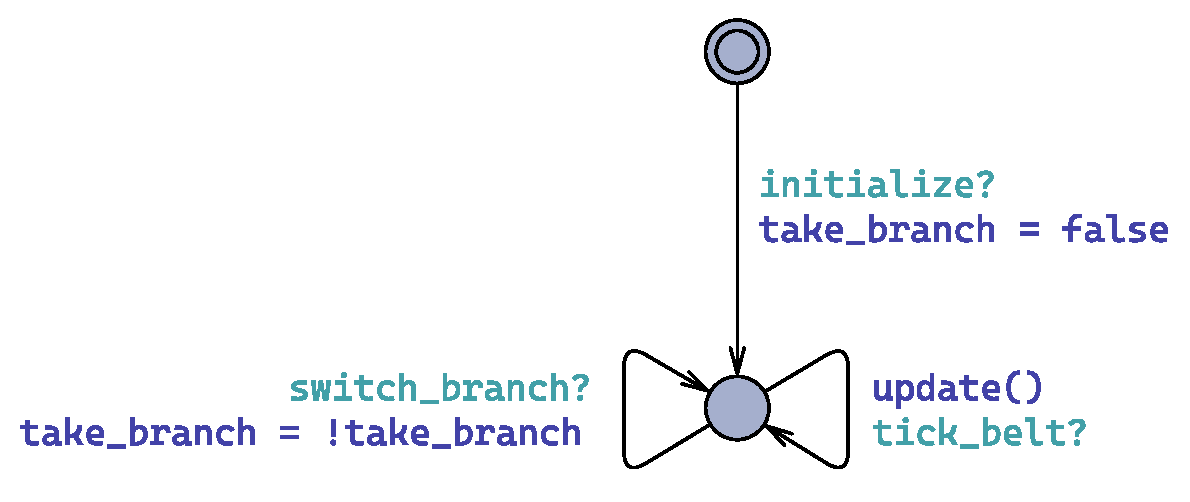
\includegraphics[width=0.33\columnwidth]{./images/automata/conveyor_belt}
        \caption{the Timed Automata of the conveyor belt.}
    \end{figure}

    It's the entity which collects all the different sectors of the plant's conveyor belt. It's a small automaton since all the underlying complexity of the conveyor belt's management is hidden behind the \texttt{update()} function. This is the most complex component of our plant since manages a lot of different things.

    \paragraph{Workpieces position} Any workpiece on a non-critical position (which is any in the following situations) is moved ahead of one slot every time the \texttt{update()} function is called.

    \paragraph{Stations and sensors management} Once a workpiece passes the input sensor of a station, it blocks any other workpiece wanting to proceed to the station itself until the sensor tells that the station is free and a new workpiece can flow again towards it.

    \paragraph{Queue management} Every time a workpiece is blocked in a specific location and some other one wants to proceed, the conveyor belt blocks it until the first one is free to move again. Since we are scanning the belt from the last positions backward this situation is easily managed since we can't place a workpiece on top or another one.

    \paragraph{Conveyor belt branch and merge} Because of the \texttt{switch\_branch?}, we keep track of the selected branch where to send the workpieces. This allows us to directly use the \texttt{update()} function to move the workpieces on the correct branch. Also, the merge of the two branches is (easily) managed by the conveyor belt, since, by scanning it backward, once we move a piece in the merge position of the belt (the one coming from the alternative branch, if any), no other one can be put in the same place, thus, blocking it from proceeding, which is exactly what happens in reality.

    \subsection{Processing stations (\texttt{Station})}

    \begin{figure}[h!]
        \centering
        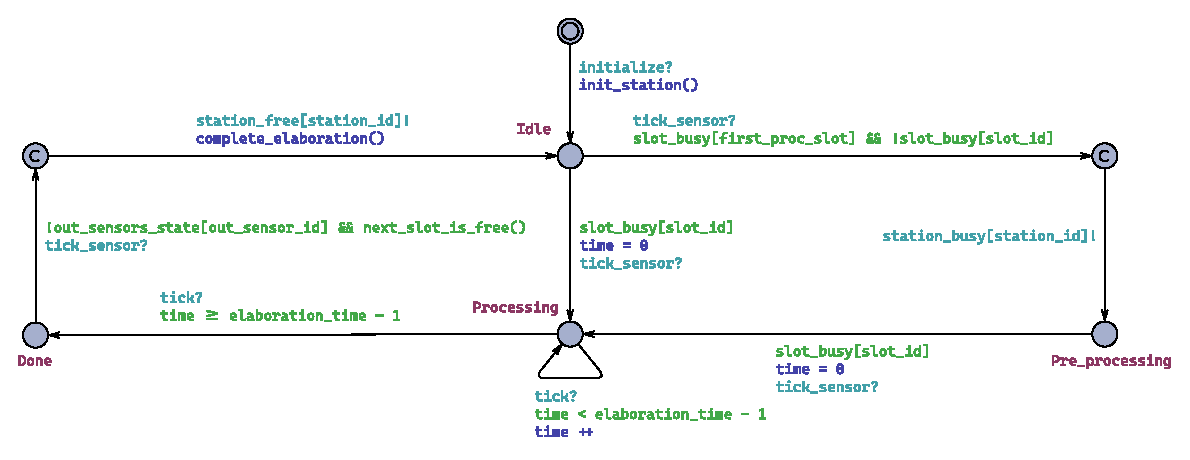
\includegraphics[width=0.84\columnwidth]{./images/automata/station}
        \caption{the Timed Automata of every station.}
    \end{figure}

    The stations model the various processes the workpieces need to go through during production. The automaton is divided in four different main states, each one of the for a different portion of the processing.

    \paragraph{Idle} This is the main state of the station, in which it doesn't have to perform any action but to wait for a workpiece to be ready for the processing.

    \paragraph{Preprocessing} When the laser sensors which is guarding the entrance of the station signals that a workpiece is approaching to it, the station moves to this state waiting for the workpiece to be in the right position.

    \paragraph{Processing} Once the workpiece is in the right position, the station starts processing it. In the model, the automaton isn't performing any real task on the workpiece, but it's simply waiting for its processing time to pass. In order to improve verification performance, we discretized the time, and so we use a counter synchronized with the global clock in order to model the time passing.

    \paragraph{Done} Once the processing time is elapsed, the station moves to this state where it waits for the right time to release the workpiece on the conveyor belt. It synchronizes with the conveyor belt itself and with the sensors guarding the entrance queue of the following station in order to know if the workpiece needs to be release or hold inside the station itself. Once the workpiece is released, the station returns to its \textit{idle} state waiting for the next processing cycle.

    \subsection{Processing station's input guard (\texttt{InSensor})}

    \begin{figure}[h!]
        \centering
        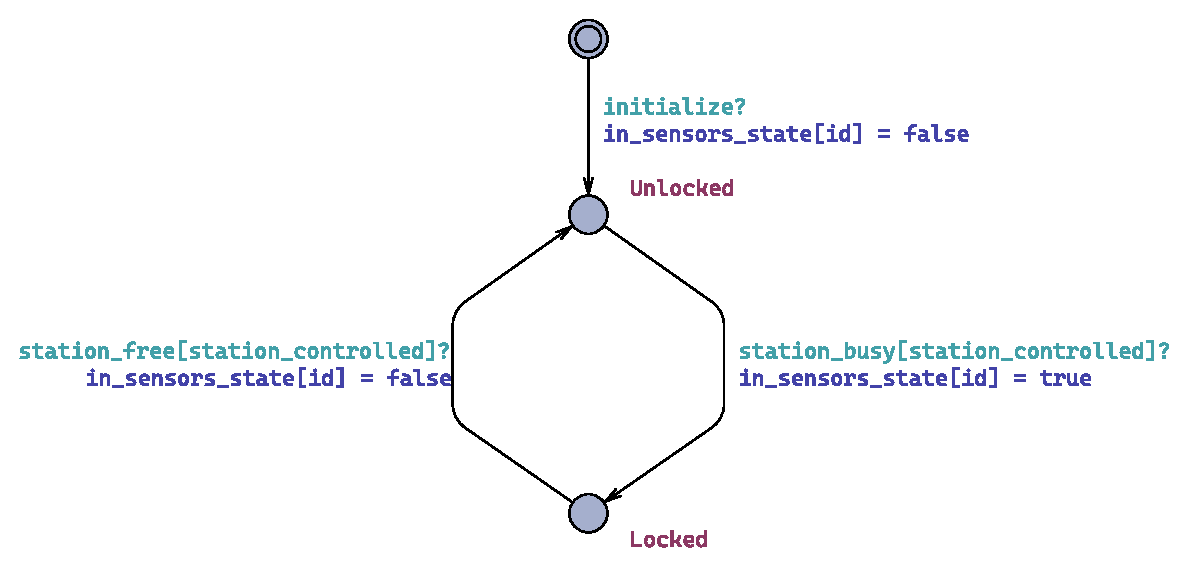
\includegraphics[width=0.5\columnwidth]{./images/automata/in_sensor}
        \caption{the Timed Automata of every input sensor.}
    \end{figure}

    These are the laser sensors that guards the entrance of a specific station. If a workpiece oversteps it, the laser sensor is equipped with a physical barrier which blocks any other following workpiece from proceeding towards the station itself until the station is free again.

    \subsection{Queue's guard (\texttt{OutSensor})}

    \begin{figure}[h!]
        \centering
        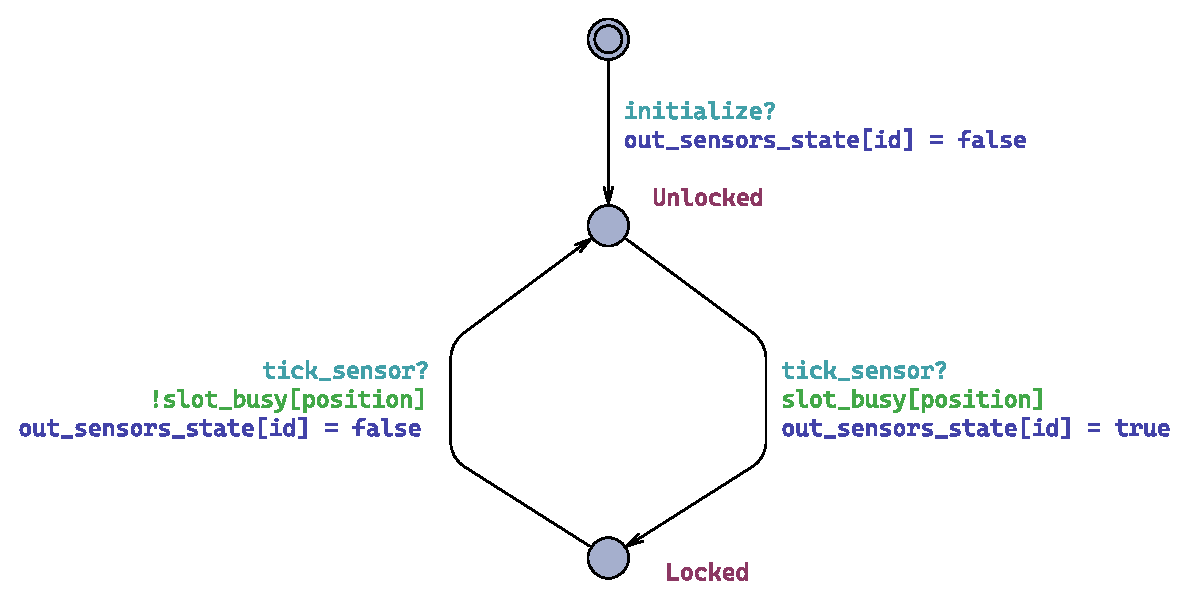
\includegraphics[width=0.45\columnwidth]{./images/automata/out_sensor}
        \caption{the Timed Automata of every output sensor.}
    \end{figure}

    Right before a station there is an \texttt{InSensor} which guards its entrance, but there may also be another sensor before it which guards the queue. Once the station's guard blocks a workpiece, others may arrive forming a queue of workpieces. This queue may have a maximum length. If the queue reaches its maximum, the sensor blocks the preceding station from releasing a workpiece if it contains one until the queue is no more full.

    \pagebreak

    \subsection{Flow controller (\texttt{FlowController\_*})}

    \begin{figure}[h!]
        \centering
        \begin{tabularx}{\linewidth}{*{2}{>{\centering\arraybackslash}X}}
            \begin{subfigure}{\linewidth}
                \caption{Controller v0}
            \end{subfigure} &
            \begin{subfigure}{\linewidth}
                \caption{Controller v1}
            \end{subfigure} \\
            \begin{subfigure}{0.5\columnwidth}
                \centering
                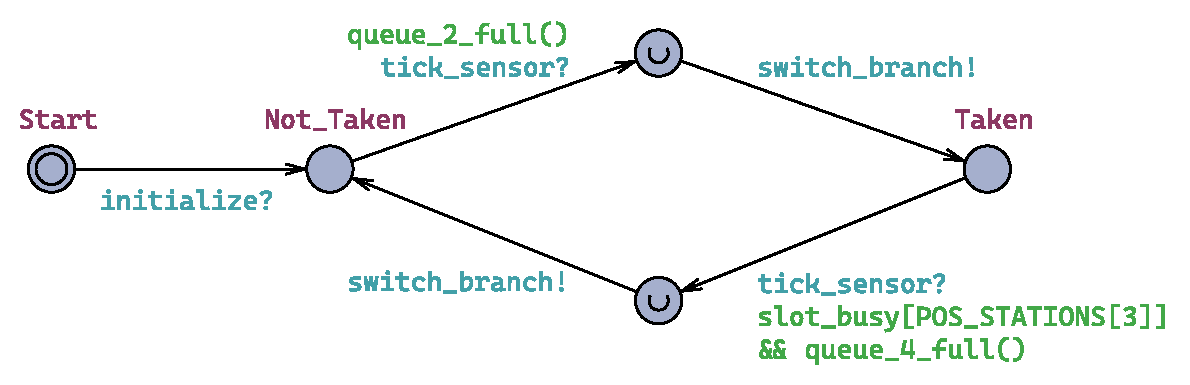
\includegraphics[width=\columnwidth]{images/automata/flow_controller_0}
            \end{subfigure} &
            \begin{subfigure}{0.23\columnwidth}  
                \centering
                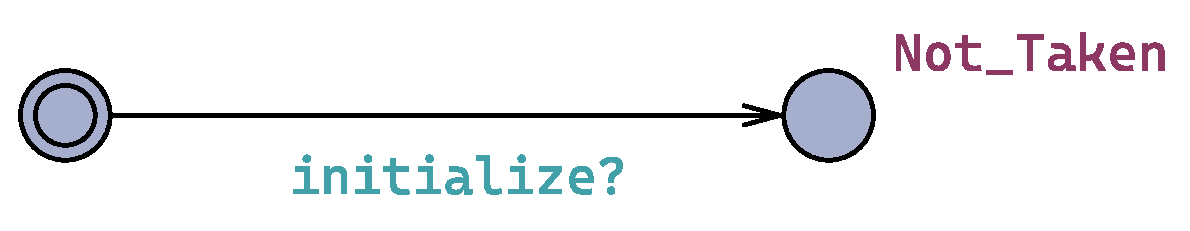
\includegraphics[width=\columnwidth]{images/automata/flow_controller_1}
            \end{subfigure} \\
            \begin{subfigure}{0.27\columnwidth}   
                \centering 
                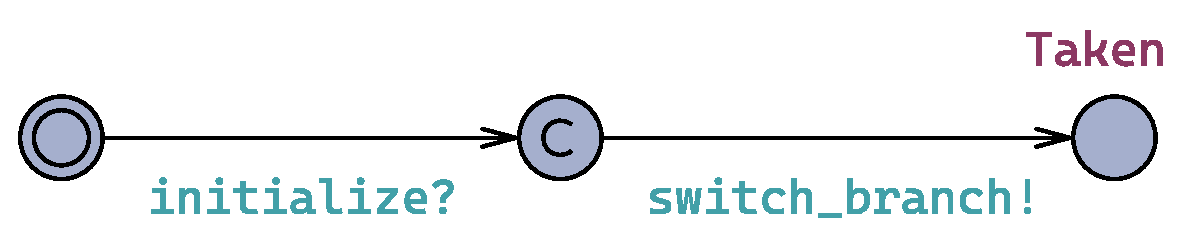
\includegraphics[width=\textwidth]{images/automata/flow_controller_2}
            \end{subfigure} &
            \begin{subfigure}{0.45\columnwidth}   
                \centering 
                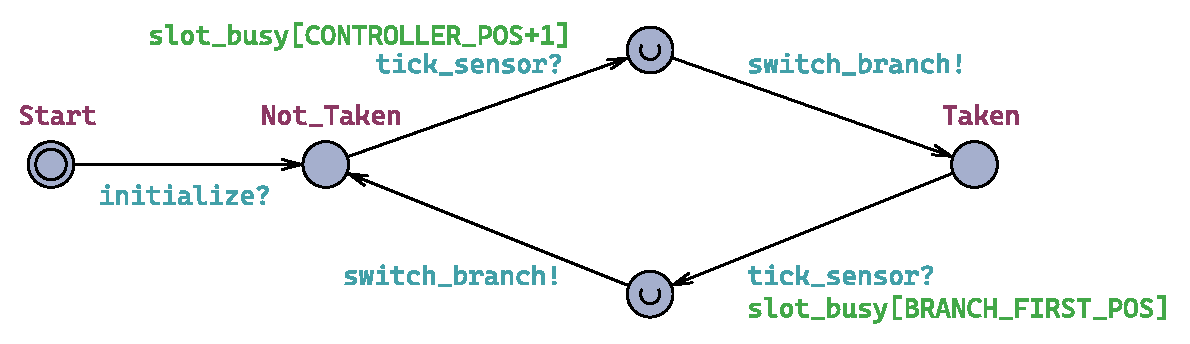
\includegraphics[width=\columnwidth]{images/automata/flow_controller_3}
            \end{subfigure} \\
            \begin{subfigure}{\linewidth}
                \caption{Controller v2}
            \end{subfigure} &
            \begin{subfigure}{\linewidth}
                \caption{Controller v3}
            \end{subfigure}
        \end{tabularx}
        \caption{the Timed Automata of the various types of controllers.}
    \end{figure}

    As explained in the introduction, these are the various policy schedules we implemented. Each one of them represents a different way to schedule the workpieces on the processing stations. Starting from the easiest ones, the ones in which all the workpieces follow the same path (either the direct one or the alternative one), to more complex ones, like the one in which we keep track of the queues in front of the first stations of the branch.\medskip

    Since the real movement of the various workpieces is managed by the conveyor belt, these automata, if they need to change the branch where the workpieces need to be sent, send a message to it in order to notify the change in the path.
    
    \section{Design Decisions} \label{section:design_decisions}

    \subsection{Hypothesis}

    \paragraph{TODO} Hypothesis (numbering, flow controller, maximum number of disks\dots).

    \subsection{Optimizations}

    Here we present all the main optimization steps we performed in order to have the final model.

    \subsubsection{The basic idea}

    \paragraph{Idea} At first, we decided to model every single entity of the plant. We had the template for generating all the single slots of the conveyor belt. This has been done in order to have a precise (and discrete) representation of the plant pointing out all the atomic components that we have.

    \paragraph{Situation} The main issue with this representation is the fact that by doing this, we had a huge verification time created by the huge number of entities and states the software had to process each time.

    \subsubsection{Unique conveyor belt}

    \paragraph{Idea} In order to simplify the modelling of the plant and our code, we decided to group all together the various slots of the conveyor belt into a logically single entity (the \texttt{ConveyorBelt}).

    \paragraph{Situation} This simplified a lot the management of all the various cases (and indeed is still present in our project) since we have a unique entity which manages all the complexity deriving from the movement of the various workpieces. This also works in synchronicity with the various processing stations and sensors in order to block the pieces when needed (and not only when there is a workpiece in front that doesn't move) and with the flow controller which tells the \texttt{ConveyorBelt} where to send the workpieces on the branch. By doing this we also improved a lot the verification time needed to check the properties, but we still had a huge memory consumption.

    \subsubsection{Unique clock}

    \paragraph{Idea} By talking with some colleagues and with the instructors we realized that we had 7 different clocks inside our project (one for the general clock of the system and one for each station) and that they tend to be one of the biggest bottlenecks during the verification phase, we decided to reduce them to just a general one, and to have all the various templates synchronizing with it.

    \paragraph{Situation} We added a new template, the \texttt{Motor}, which sends the right signals at the right moment to all the components that need it respecting the speed of the conveyor belt's movement, and we synchronized the stations' processing times with the general clock of the system (which is not related to the speed of the conveyor belt). By doing this we reduced the number of possible transitions the system can take at any instance, and we make sure that everything is synchronized with just one single entity. This allowed us to have a skyrocketing verification time, even with 12 different workpieces circulating in the production plant at the same time.

    \section{Properties}

    \paragraph{TODO} Properties we are verifying (in TCTL and not in UPPAAL's language).

    \section{Stochastic version}

    \paragraph{TODO} Explain it and point out the differences with the automata we changed.

    \section{Scenarios}

    These are some possible scenarios which want to show that the production plant we modelled works correctly in any (normal) situation. There are some pathological cases in which the plant fails to guarantee some properties, but it's completely normal since they are all pathological cases. Some of them are depicted here.

    \subsection{Scenario 1: the normality}

    This is a general scenario in which the structure of the plant is the same as the one depicted in the introduction. The stations' processing times have been chosen without any specific criterion, and we instructed the flow controller to equally send the workpieces on the two different branches of the conveyor belt (each one on the opposite branch with respect to the previous workpiece).

    \paragraph{Parameters}

    \begin{center}
        \begin{tabular}{|c|c|c|c|c|}
            \hline
            {\fontfamily{lmtt}\fontseries{b}\selectfont SPEED} & {\fontfamily{lmtt}\fontseries{b}\selectfont DISKS} & \textbf{Policy} & {\fontfamily{lmtt}\fontseries{b}\selectfont POS\_OUT\_SENSORS} & {\fontfamily{lmtt}\fontseries{b}\selectfont STATIONS\_ELABORATION\_TIME} \\
            \hline
            1 & 12 & 3 & [2, 24, 68, 90, 105] & [6, 7, 8, 9, 8, 7] \\
            \hline
        \end{tabular}
    \end{center}

    \paragraph{Simulations} This is what we obtained by simulating the system for 1000 time instants:

    \begin{figure}[h!]
        \begin{subfigure}{\textwidth}
            \centering
            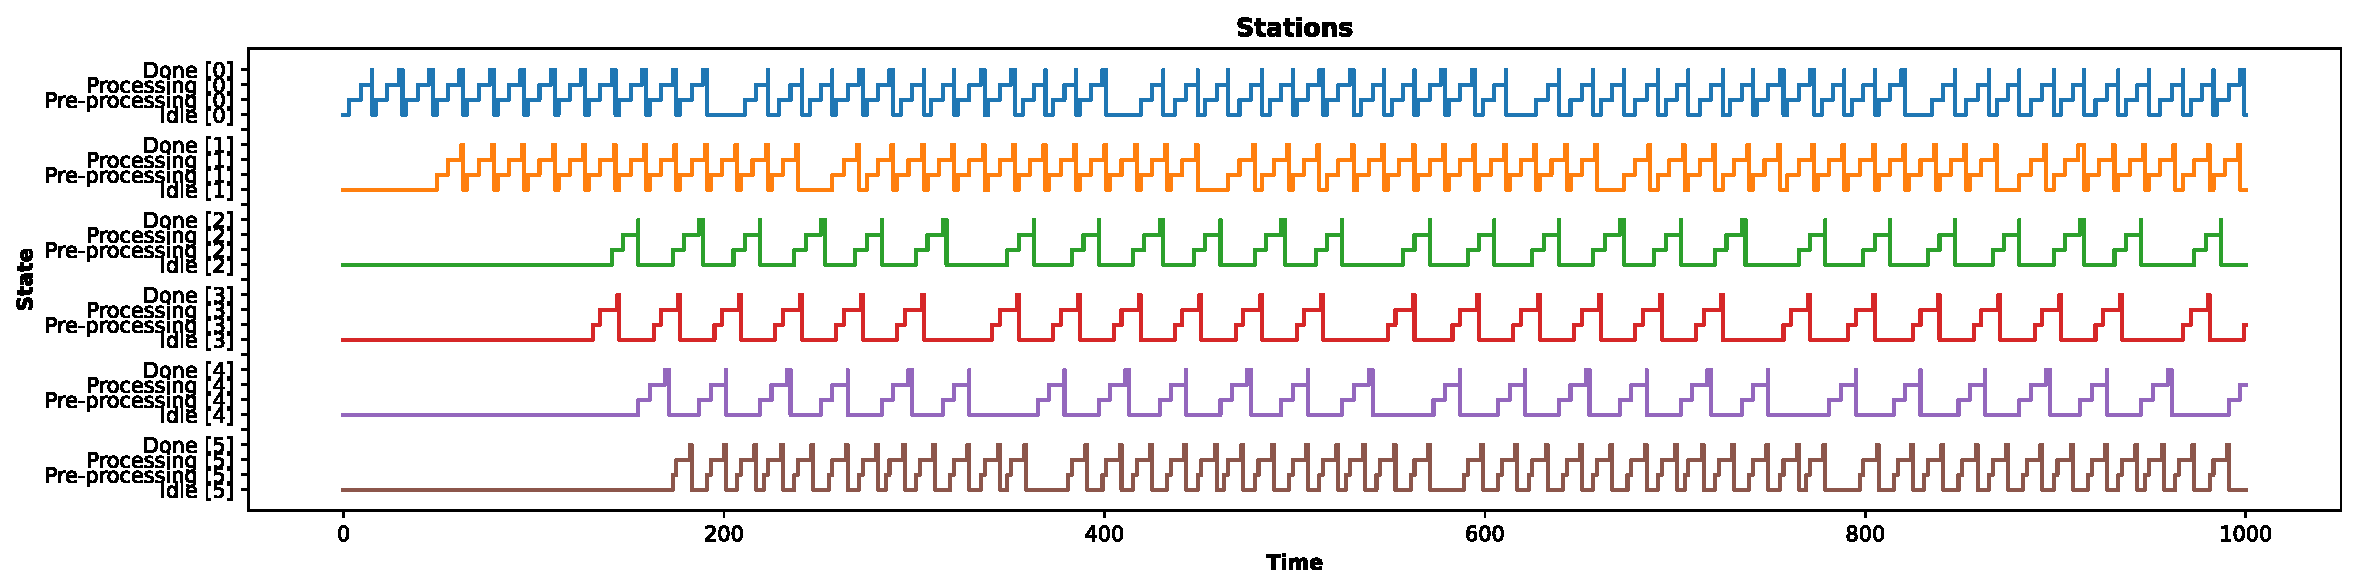
\includegraphics[width=0.9\textwidth]{images/scenarios/scenario1_stations}
        \end{subfigure}
        \begin{subfigure}{0.49\textwidth}
            \centering
            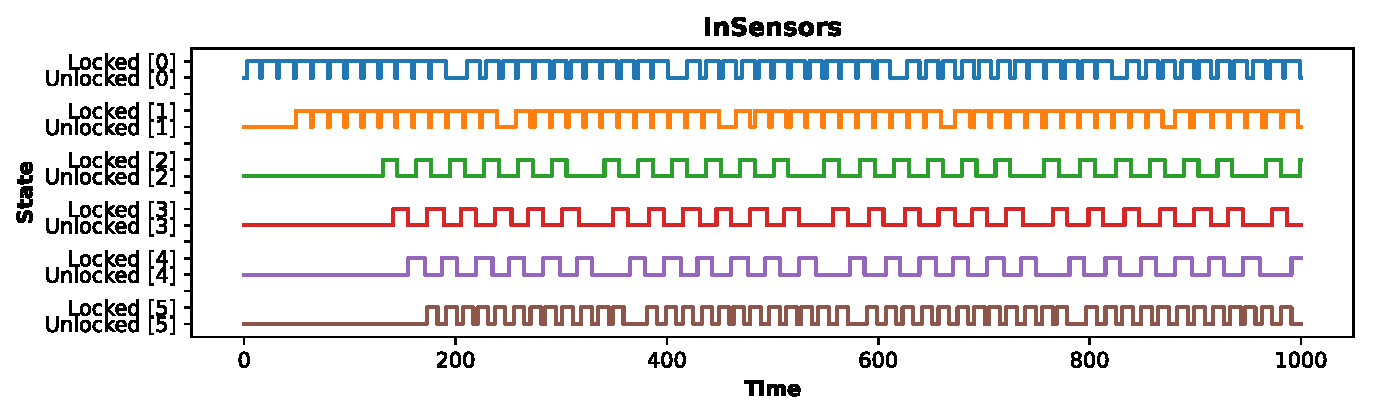
\includegraphics[width=\textwidth]{images/scenarios/scenario1_insensors}
        \end{subfigure}
        \hfill
        \begin{subfigure}{0.49\textwidth}
            \centering
            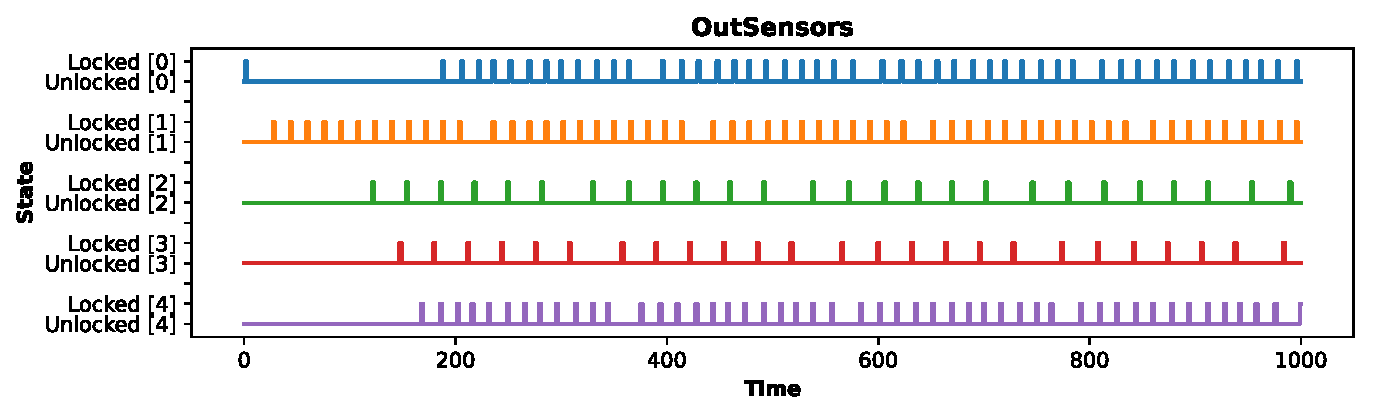
\includegraphics[width=\textwidth]{images/scenarios/scenario1_outsensors}
        \end{subfigure}
        \caption{the results of the simulation over 1000 time instants.}
    \end{figure}

    \paragraph{Results} All the properties are \textit{verified}. As it's supposed to, the plant is working without any problem and all the workpieces flow all around the plant without any problem. The sensors are guaranteeing the required properties and the stations do their job flawlessly.

    \subsection{Scenario 2: short queues}

    With this scenario we want to test if the plant is working in a normal production situation (in which all the processing times of the various stations are balanced), but with short queues in front of the various stations.

    \paragraph{Parameters}

    \begin{center}
        \begin{tabular}{|c|c|c|c|c|}
            \hline
            {\fontfamily{lmtt}\fontseries{b}\selectfont SPEED} & {\fontfamily{lmtt}\fontseries{b}\selectfont DISKS} & \textbf{Policy} & {\fontfamily{lmtt}\fontseries{b}\selectfont POS\_OUT\_SENSORS} & {\fontfamily{lmtt}\fontseries{b}\selectfont STATIONS\_ELABORATION\_TIME} \\
            \hline
            1 & 12 & 3 & [12, 33, 76, 92, 106] & [2, 15, 5, 3, 2, 5] \\
            \hline
        \end{tabular}
    \end{center}

    \paragraph{Simulations} This is what we obtained by simulating the system for 1000 time instants:

    \begin{figure}[h!]
        \begin{subfigure}{\textwidth}
            \centering
            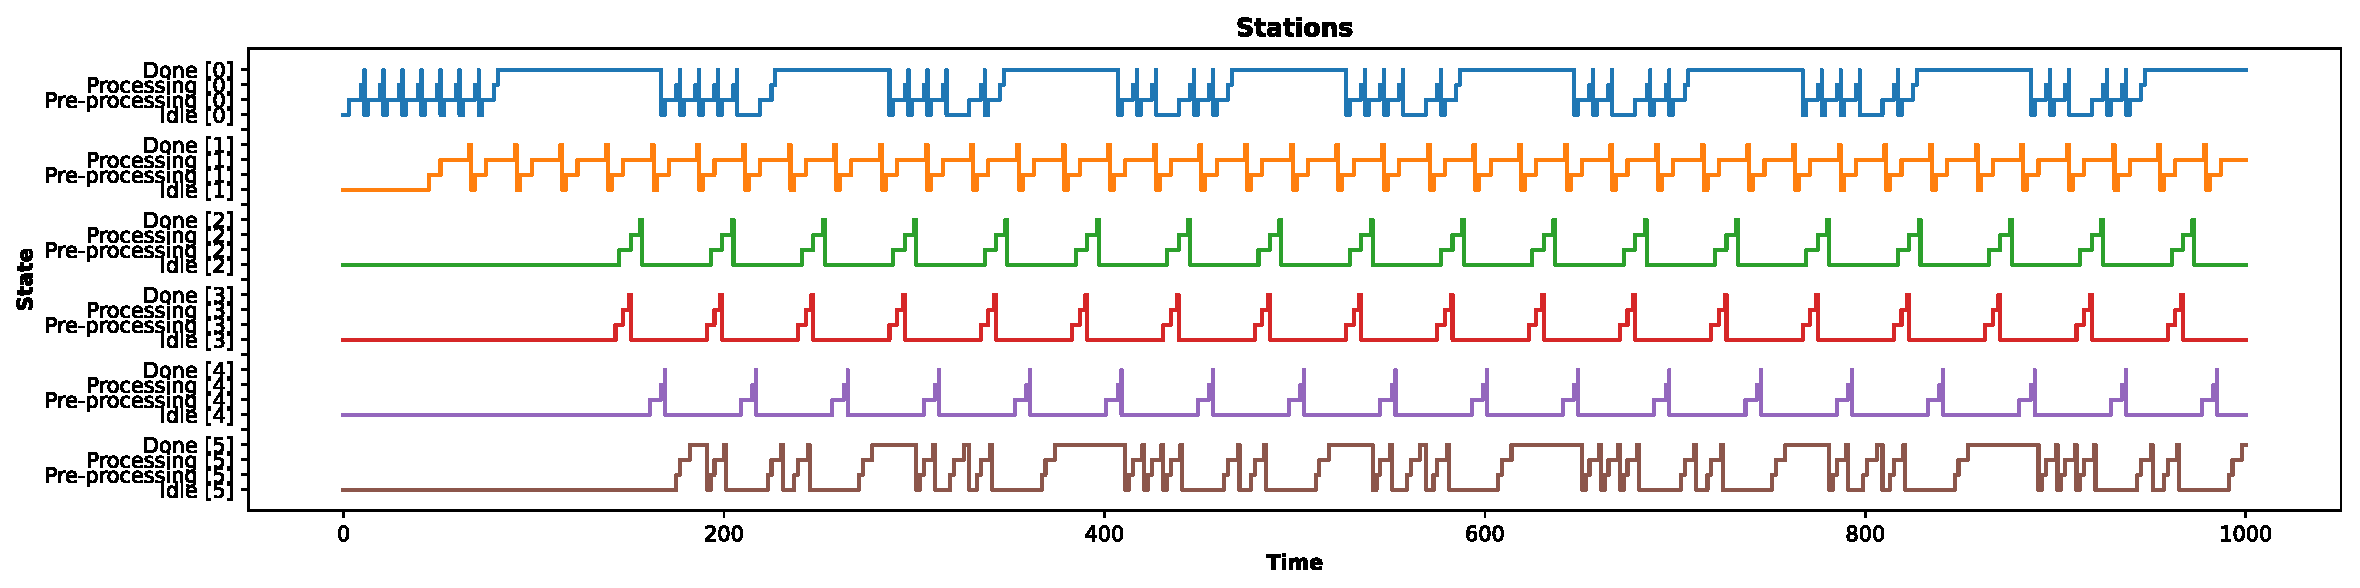
\includegraphics[width=0.9\textwidth]{images/scenarios/scenario2_stations}
        \end{subfigure}
        \begin{subfigure}{0.49\textwidth}
            \centering
            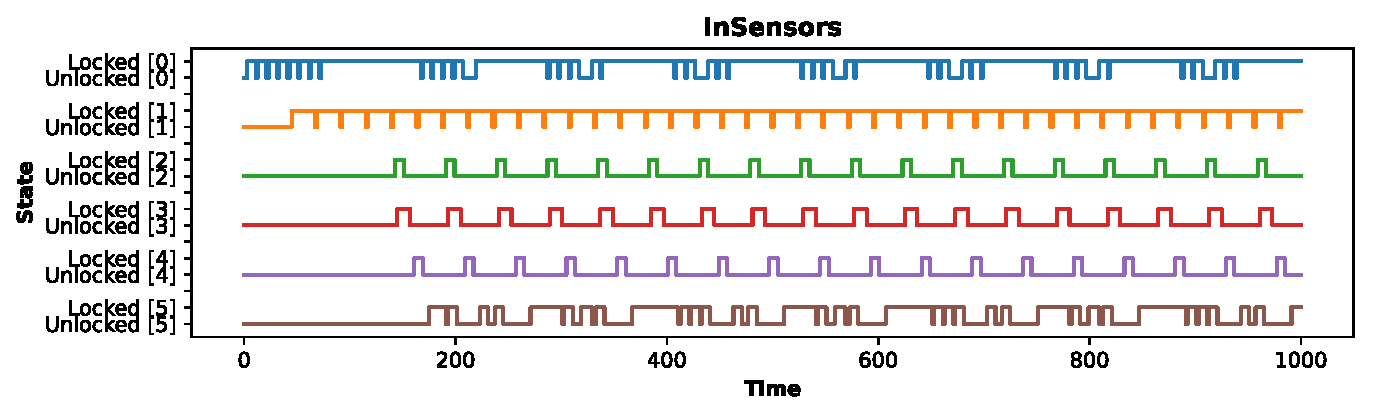
\includegraphics[width=\textwidth]{images/scenarios/scenario2_insensors}
        \end{subfigure}
        \hfill
        \begin{subfigure}{0.49\textwidth}
            \centering
            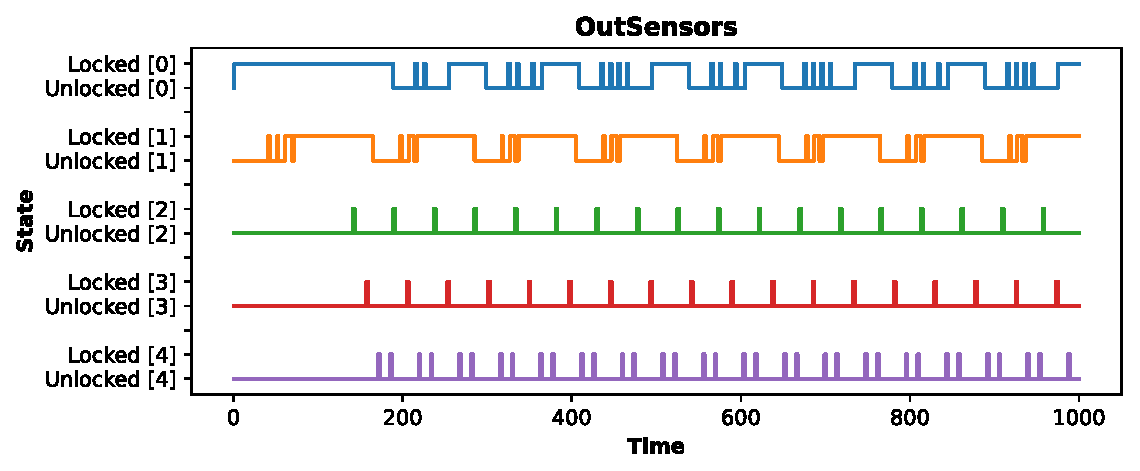
\includegraphics[width=\textwidth]{images/scenarios/scenario2_outsensors}
        \end{subfigure}
        \caption{the results of the simulation over 1000 time instants.}
    \end{figure}

    \paragraph{Results} All the properties are \textit{verified}. The graphics show us that the system is working correctly without any particular delay on the stations.
    
    \paragraph{Particular case} If we try to play a bit with the processing times of the stations, we can create a situation where station 2 and 4 release a piece in such a way that they saturate the queue in front of station 5, exceeding its limit. An example could be a very short processing time on the first two stations in order to let the workpieces flow, the same overall time on the two branches, and very long one at the last station. In this way we break the third property, but it's completely expected, since the plant is not smart enough for preventing this situation to happen.

    \subsection{Scenario 3: one way}

    Here we wanted to test a different scheduling policy. In particular, we choose to route all the workpieces through the branch with the two processing stations. The only thing we changed with respect to the first scenario is the scheduling policy.

    \paragraph{Parameters}

    \begin{center}
        \begin{tabular}{|c|c|c|c|c|}
            \hline
            {\fontfamily{lmtt}\fontseries{b}\selectfont SPEED} & {\fontfamily{lmtt}\fontseries{b}\selectfont DISKS} & \textbf{Policy} & {\fontfamily{lmtt}\fontseries{b}\selectfont POS\_OUT\_SENSORS} & {\fontfamily{lmtt}\fontseries{b}\selectfont STATIONS\_ELABORATION\_TIME} \\
            \hline
            1 & 12 & 2 & [2, 24, 68, 90, 105] & [6, 7, 8, 9, 8, 7] \\
            \hline
        \end{tabular}
    \end{center}

    \paragraph{Simulations} This is what we obtained by simulating the system for 1000 time instants:

    \begin{figure}[h!]
        \begin{subfigure}{\textwidth}
            \centering
            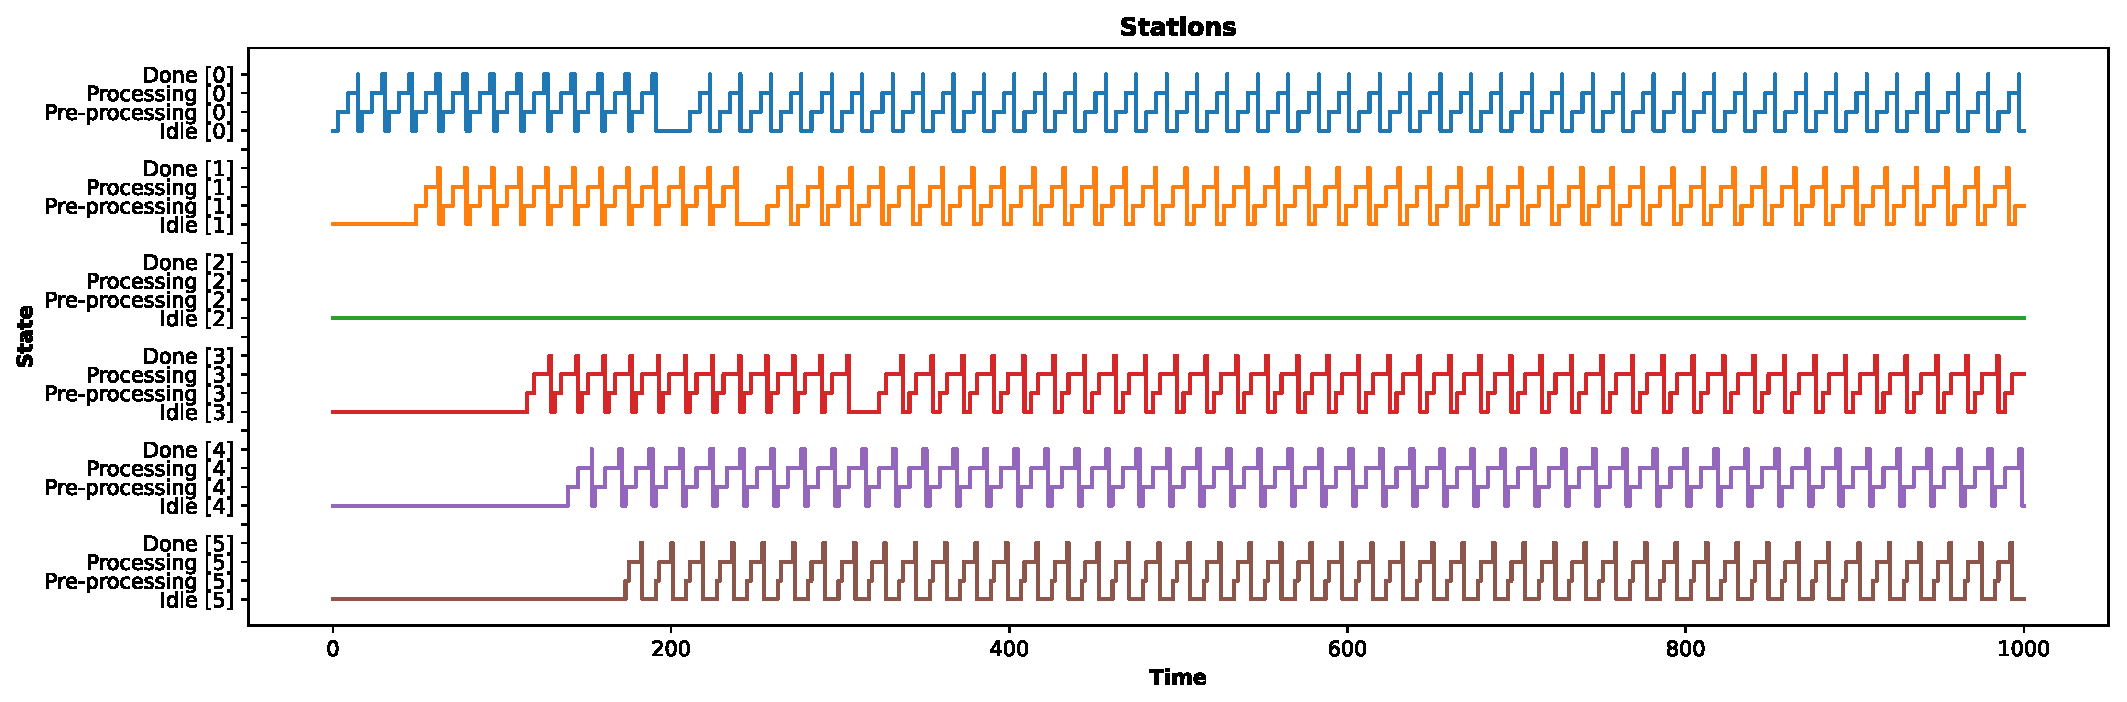
\includegraphics[width=0.9\textwidth]{images/scenarios/scenario3_stations}
        \end{subfigure}
        \begin{subfigure}{0.49\textwidth}
            \centering
            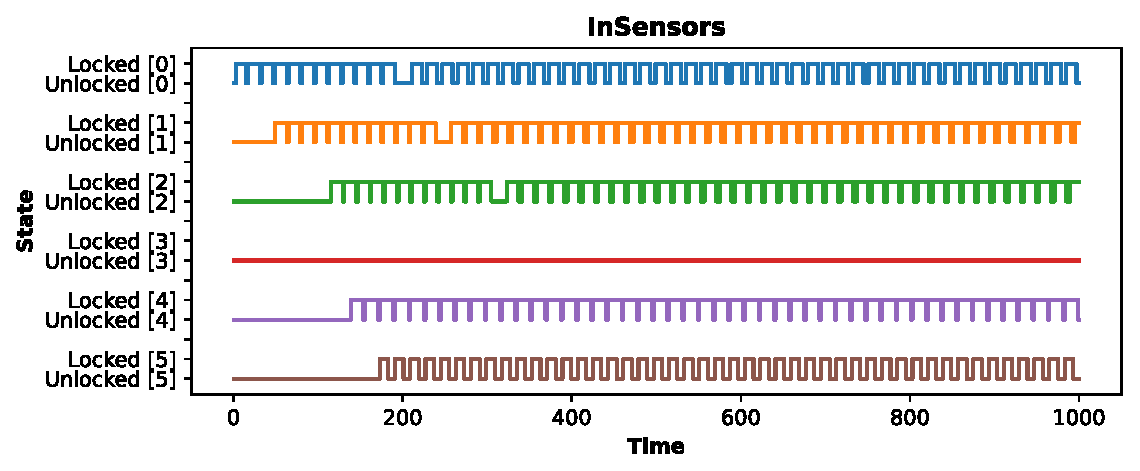
\includegraphics[width=\textwidth]{images/scenarios/scenario3_insensors}
        \end{subfigure}
        \hfill
        \begin{subfigure}{0.49\textwidth}
            \centering
            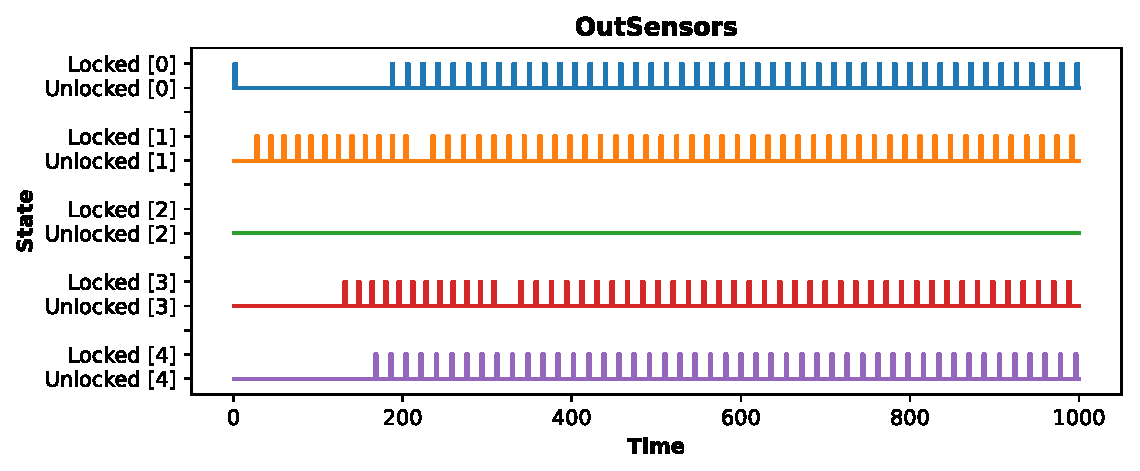
\includegraphics[width=\textwidth]{images/scenarios/scenario3_outsensors}
        \end{subfigure}
        \caption{the results of the simulation over 1000 time instants.}
    \end{figure}

    \paragraph{Results} All the properties are \textit{verified}. If we take a closer look to the graphics, and we compare them with the ones of the first scenario, we can notice that the scheduling policy in which we divide the workpieces on the two different branches (so the one of the first scenario) is slightly more efficient than this one (station 0 here processes 56 pieces in 1000 time instants with respect to the 58 ones of the first scenario), which may be expected since, usually, balancing the workload is the best solution.

    \subsection{Scenario 4}

    \subsection{Scenario 5 (stochastic)}

    \subsection{Scenario 6 (stochastic)}

    \section{Conclusions}

\end{document}
